\documentclass{beamer}
\usetheme{Warsaw}
\usepackage{nhtvslides}
\usepackage{graphicx}
\usepackage{amssymb}
\usepackage{pifont}
\usepackage{listings}
\lstset{language=CAML,
basicstyle=\ttfamily\footnotesize,
frame=shadowbox,
breaklines=true,
mathescape=true}
\usepackage[utf8]{inputenc}

\newcommand{\cmark}{\ding{51}}%
\newcommand{\xmark}{\ding{55}}%

\title{LGOAP}
\subtitle{Adaptive layered planning for real-time video games}

\author{Dr. Giuseppe Maggiore}

\institute{NHTV University of Applied Sciences \\ 
Breda, Netherlands}

\date{}

\begin{document}
\maketitle

\begin{frame}{Agenda}
\tableofcontents
\end{frame}

\section{Introduction}
\begin{slide}{NPCs in games}{Realism}{
\item Non-playing characters (NPCs) in modern games often exhibit behavior that is strategically and tactically inferior
\item In general, NPC behaviour is clearly artificial and unrealistic
}\end{slide}

\begin{slide}{NPCs in games}{Realism}{
\item We wish NPCs who are part of the game world as much as the player is
\item They should \textit{play} the game rather than \textit{be a passive part} of it
\item Anything that the player can do, NPCs should be able to do as well
}\end{slide}

\begin{slide}{NPCs in games}{Realism}{
\item NPCs should be able to recognize the actions available to them
\item NPCs should choose the best course of action because it makes sense according to their internal logic...
\item ...either to fulfill their needs or to reach some goal
}\end{slide}

\begin{textslide}{NPCs in games}{Problem statement}{
\textbf{To what extent can planning be used to create adaptive behaviour of NPCs that allows them to achieve long and short term goals in a real-time game or simulation?}
}\end{textslide}

\begin{slide}{NPCs in games}{Idea}{
\item \textit{create and execute, in real-time, plans that consist of sequences of actions}
\item Actions are defined as transitions in the game world state
\item Multiple actions are available to an NPC in a given state, but only one can be chosen for the final plan
\item We define the game world as a distribution of resources over entities and agents
\item Actions cause only changes to that distribution
\item This allows us to consider actions as transitions in a graph, across which the planner finds an optimal path in order to reach the desired state
}\end{slide}

\begin{slide}{NPCs in games}{Idea, part 2}{
\item how do we model an abstract game world so that the approach works on any concrete game world without modification?
\item what search algorithm can we use that can be executed sufficiently fast?
\item how can we deal with NPC personalization?
\item how can we deal with the fact that an NPC can only plan his own actions, while the future world state depends on the actions of all NPCs?
}\end{slide}

\section{Ontology of actions}
\begin{slide}{Ontology of actions}{Entities, resources, actions}{
\item We define the game world as a series of \textit{entities} (such as a table, a chair, a gun, a gem, etc.) 
\item A series of \textit{agents} are the playing and non-playing characters
\item Entities may change dynamically: their locations may vary and they may be added or removed from the game world
\item All entities contain \textit{resources} (or \textit{stats})
\item All agents contain resources as well
\item When an agent interacts with an entity, it does so by activating an \textit{action}
\begin{itemize}
\item An action exchanges resources between entities and agents
\item Actions may change dynamically and may be added or removed
\end{itemize} 
}\end{slide}

\begin{frame}[fragile]{Simple example}
\begin{lstlisting}
L=life        Sword      Agent      Ogre
A=attack       L=1        L=5        L=5
*=entity       A=2        A=0        A=1       Goal
-=tile          *----------*----------*----------*
\end{lstlisting}
\end{frame}

\begin{slide}{Ontology of actions}{Entities, resources, \textbf{actions}}{
\item \texttt{Sword.pickup}, which increases the attack rating of the agent who picks it up and decreases the life of the sword;
\item \texttt{Tile.walk} that changes the current location of an agent;
\item \texttt{Ogre.fight} that subtracts the attack resource of the agent from the life resource of the ogre and vice-versa.
}\end{slide}

\begin{textslide}{Ontology of actions}{Example run}{
Example run
}\end{textslide}

\begin{slide}{Ontology of actions}{Entities, resources, actions}{
\item Extensions without much effort
\item For example, we could add a new resource, \texttt{key}
\item We can now add a room to the dungeon which requires a key in order to obtain the sword
}\end{slide}

\begin{frame}[fragile]{Extended example}
\begin{lstlisting}
L=life                 Agent      Ogre
A=attack     Key        L=5        L=5
K=key        K=1        A=0        A=1       Goal
*=entity      *----------*----------*----------*
_=tile                   |
                         | Door
                         *  K=1
                         |
                         | Sword
                         *  A=2
\end{lstlisting}
\end{frame}

\begin{slide}{Ontology of actions}{New actions}{
\item \texttt{Key.pickup}, which adds to an agent a key resource
\item \texttt{Door.open}, which subtracts from the door key resource the agent's key resource
}\end{slide}

\begin{textslide}{Ontology of actions}{Example run}{
Example run
}\end{textslide}

\begin{slide}{Ontology of actions}{Constraint logic programming}{
\item Framework connected to \textit{constraint logic programming} \cite{CONSTRAINT_PROGRAMMING}
\item Actions change the resources of the various entities of the game world if some preconditions are met
}\end{slide}

\begin{frame}[fragile]{\texttt{Sword.pickup}}
\begin{lstlisting}
Agent.L > 0 $\wedge$ Sword.L > 0 $\wedge$ Agent.P = Sword.P $\rightarrow$ Sword.L := 0 $\wedge$ Agent.A := Agent.A + 2
\end{lstlisting}
\end{frame}

%\begin{textslide}{Ontology of actions}{Constraint logic programming}{
%Example run of CLP
%}\end{textslide}

\section{Planning}
\begin{slide}{Planning}{Event horizon}{
\item A game state is a distribution of resources over entities and agents
\item Actions move the game world from one state to another
\item Current NPCs blindly pick one action at a time, without considering the medium and long term consequences of their decisions
\item Planning solves this problem by giving the AI the ability to select \textit{sequences} of actions
}\end{slide}

\begin{slide}{Planning}{Planning as path-fiding}{
\item Such a planning algorithm is a (multi-dimensional) path-finder
\item Explore a large graph where:
\begin{itemize}
\item Nodes are \textit{all} the valid states of the game world
\item Actions represent transitions from one of the valid states into another one
\item The new state of the game world will be forward in time
\item As a result of the actions used it will have different resources, entities, and available actions
\end{itemize}
\item Graph exploration techniques are connected to planning \cite{STATE_SPACE_SEARCH}
}\end{slide}

\begin{slide}{Planning}{Naïve planning}{
\item Planning in a game can be done naïvely with backtracking on all the possible sequences of actions
\item Backtracking ends after a satisfactory plan is found
\item Appropriate failure conditions must be taken into account (upper bound on number of actions, timeout, etc.)
}\end{slide}

\begin{frame}[fragile]{Naïve planning}
\begin{lstlisting}
find_plan(world,agent,steps) =
  if length(steps) > MAX_STEPS then
    return null
  if goal_reached(world,agent) then
    return steps
  else
    for action in available_actions(world,agent) do
      world',agent' = simulate_action(world,agent,action)
      result = find_plan(world',action',action::steps)
      if result <> null then
        return result // this plan reaches the goal
    return null // failure
\end{lstlisting}
\end{frame}

\begin{slide}{Planning}{Cost of naïve planning}{
\item Back-tracking is effective but inefficient
\item Assume that at every step there are at least $A$ actions available
\item Assume that plans with more than $N$ actions are discarded
\pause
\item Every possible sequence of actions of length $N$ may be explored
\item The complexity of the algorithm is $O(A^N)$
\item This number will quickly become too large to be feasible
}\end{slide}

\begin{slide}{Planning}{Optimization}{
\item Heuristic search \cite{HEURISTIC_SEARCH}: a less wasteful variation of backtracking
\item Some \textit{inferior} plans are not explored at all
Take into account the resource constraints of the possible actions \cite{HEURISTIC_PLANNING_WITH_RESOURCES}
\item Steer the planner towards plans that maintain desirably high levels of certain important resources
\item Steer the planner towards a given goal
\item For example, a plan that reduces the \texttt{health} of an NPC to zero can safely be ignored
}\end{slide}

\begin{slide}{Planning}{Path-finding}{
\item A graph containing all reachable game worlds is too large to warrant straightforward exploration
\item Cannot use Dijkstra's algorithm
\item We can use \textit{iterative deepening depth-first search} (IDDFS) \cite{IDDFS}
\item Each iteration increases the depth of exploration until the shallowest goal state is reached
\item IDDFS is a form of breadth-first search
\item In particular, we use IDA* \cite{IDAStar}
}\end{slide}

\begin{slide}{Planning}{IDA*}{
\item IDA* is an informed search, because it expands the reached nodes according to some heuristic
\item A node represents a possible state of the game world
\item We pick and expand the \textit{most desirable} state 
\item The desirability of a game world is a heuristic which may vary depending on the specific scenario
\item For example, an ordering of the NPC resources
}\end{slide}

\begin{slide}{Planning}{IDA*}{
\item This heuristic drive has two side-effects: \textit{(i)} finds plans that satisfy the goal while optimizing some resources; and \textit{(ii)} speed up the search process by focusing on promising states
\item Further speed up: trim the set of working plans to a maximum size
\item Warning: trade-off between search thoroughness and speed
\item Smaller working set means faster
\item Too small working set may cull (temporarily bad) plans
}\end{slide}

\begin{frame}[fragile]{Heuristic search}
\begin{lstlisting}
find_plan_fast(world,agent) =
  Q = {(world,agent)}
  C = 0
  do
    if $\exists$ p $\in$ Q : reaches_goal(p) then
      return p
    Q $\leftarrow$ { simulate_action(p,a) : p $\in$ Q $\wedge$ a $\in$ available_actions(world,agent) }
    Q $\leftarrow$ take_best_M()
  while Q $\neq$ $\emptyset$ $\wedge$ Steps < N
  return null
\end{lstlisting}
\end{frame}

\begin{slide}{Planning}{Heuristic search complexity}{
\item Resulting complexity becomes $O(N \times M \times A)$, where $M$ is the maximum size of the queue
\item Optimizations can partially mitigate slowness of the algorithm
\item Increasing the target length of plans steeply increases the computation time required
\item Unfortunately, we need long plans
}\end{slide}

\begin{slide}{Planning}{Hierarchy of planners}{
\item Further reduce complexity 
\item Hierarchical system similar to \cite{HIERARCHICAL_PLANNING}
\item Multiple planners nested inside one another
\item Highest level planners actions span a long time
\item Each action involves large changes in resources
\item Lower level planners find plans that respect the constraints given by the higher layers
\item Lower level actions are more concrete, take less time, and generally involve smaller resource exchanges
}\end{slide}

\begin{slide}{Planning}{Hierarchy of planners}{
\item Consdier three layers in the RPG example
\begin{description}
\item[Highest level] \texttt{complete quest X}, \texttt{acquire sword}, \texttt{fight ogre}
\item[Middle layer] \texttt{use item X}
\item[Lowest layer] \texttt{move to X}
\end{description}
}\end{slide}

\begin{slide}{Planning}{Hierarchy of planners}{
\item Final planning system invokes the fast planning function multiple times
\begin{itemize}
\item Different actions
\item Different goal
\end{itemize}
}\end{slide}

\begin{frame}[fragile]{Layered planner}
\begin{lstlisting}
find_plan_layered(world,agent) =
  plan = find_plan_fast$_L$(world,agent)
  for l = L-1 downto 0 do
    new_plan $\leftarrow$ []
    for (world,agent,action) in plan
      new_plan $\leftarrow$ find_plan_fast$_{l,action}$(world,agent) :: new_plan
    plan $\leftarrow$ new_plan
  return plan
\end{lstlisting}
\end{frame}

\begin{slide}{Planning}{Layering complexity}{
\item New algorithm has significantly decreased computational load 
\item Our planner can now plan for much longer periods of time
\item Algorithm invokes the fast planning algorithm once for every layer ($L$ times), and for each action found by each layer ($N$ times)
\item $O(L \times N^2 \times M \times A)$
\item Final plan, entirely composed of lowest level actions is now long $N^L$ actions
}\end{slide}

\begin{textslide}{Planning}{Complexities}{
\begin{table}
\center
\begin{tabular}{| l | p{3cm} | p{3cm} | }
\hline
Algorithm & Complexity & Steps \\
\hline
Naïve & $O(A^{T_{tgt} / T})$ & $10^{100}$ \\
Fast & $O(\frac{T_{tgt}}{T} \times M \times A)$ & $100000$ \\
Layered & $O(L \times \sqrt[L]{\frac{T_{tgt}}{T}}^2 \times M \times A)$ & $15000$ \\
\hline
\end{tabular}
\caption{Steps per algorithm for $M=100$, $A=10$, ${T_{tgt}/T}=100$, $L=3$}
\label{tab:steps}
\end{table}
}\end{textslide}

\begin{slide}{Planning}{Memory}{
\item Small memory of old plans
\item Useful past plans are stored for each layer \cite{MEMOIZATION_PLANNING} (\textit{memoization} or \textit{tabling} \cite{MEMOIZATION})
\item Each plan contains a sequence of actions and some \textit{circumstances} (time, location, NPC resources)
}\end{slide}

\begin{slide}{Planning}{Memory}{
\item In case of matching circumstances, the plan is considered for re-activation
\item Results of the plan are then estimated from the current configuration
\item If the result achieves the current goal then the plan is used
\item When a plan is used, then its score is increased
\item Score determines removal/permanence of plan in memory
}\end{slide}

\begin{frame}[fragile]{Memory}
\begin{lstlisting}
recall_plan(world,agent) =
  for plan in agent.memory do
    if similar(plan.world,world) $\wedge$
       reaches_goal(plan) then
       increase_score(plan)
       return plan
  return null
\end{lstlisting}
\end{frame}

\begin{slide}{Planning}{Personalized NPCs}{
\item Our framework allows the differentiation of NPCs
\item Different NPCs make plan based on their preferences
}\end{slide}

\begin{slide}{Planning}{Personalized NPCs}{
\item NPCs now favour certain plans
\item Still, restrict to valid plans
\item Also, priority given by heuristic selection depends on preferences
\item For example, an NPC that favors magic will expand magic fighting actions
}\end{slide}

\section{Plan execution}
\begin{slide}{Execution}{Plan execution}{
\item After the planning phase plans are actually put into action
\item While planning, NPC's read and modify temporary copies of the game world state
\item The game world itself is never affected by planning
}\end{slide}

\begin{slide}{Execution}{Sequentialization}{
\item The simplest scheme just alternates planning and execution
\item Planning happens in a single tick of the simulation
\item After planning, straightforward execution executes the plan actions in order
}\end{slide}

\begin{frame}[fragile]{Sequentialization}
\begin{lstlisting}
while true do
  plan = find_plan(world,self)
  execute_plan(world,self,plan)
\end{lstlisting}
\end{frame}

\begin{frame}[fragile]{Sequentialization}
\begin{lstlisting}
execute_plan(world,self,plan) =
  for action in plan.Actions do
    execute_action(world,self,action)
\end{lstlisting}
\end{frame}

\begin{slide}{Execution}{Plan execution}{
\item We are executing plans in real-time
\item We must ensure that an executed plan remains sensible
\item Cannot predict how lower level plans will achieve goals, other agents, etc.
}\end{slide}

\begin{slide}{Execution}{Non-determinism}{
\item Long-term planning, non-determinism, or layering cause wrong expectations
\item Planning errors may be benign (a plan is yielding higher benefits than expected) 
\item Planning errors may be malign (a plan is costing more than anticipated)
\item Negative effects may add up to the point of an NPC death
\item Checks to determine if an action can be performed safely
}\end{slide}

\begin{frame}[fragile]{Non-determinism}
\begin{lstlisting}
execute_plan(world,self,plan) =
  for action in plan.Actions do
    if action.cost < agent.resources then
      execute_action(world,self,action)
    else
      return
\end{lstlisting}
\end{frame}

\begin{slide}{Execution}{Tracking expectations}{
\item We can keep track inside a plan of the expected results of each action
\item We can then check so that an NPC keeps running a plan only under the original assumptions
}\end{slide}

\begin{frame}[fragile]{Tracking expectations}
\begin{lstlisting}
execute_plan(world,self,plan) =
  for action in plan.Actions do
    if action.cost < agent.resources $\wedge$
       matched(action.expectations,world,agent) then
      execute_action(world,self,action)
    else
      return
\end{lstlisting}
\end{frame}

\begin{slide}{Execution}{Tracking expectations}{
\item NPCs can safely try and plan ahead for even multiple days or weeks of simulation time
\item Replanning will be triggered before an execution is completed if needed
}\end{slide}

\begin{slide}{Execution}{Concurrent planning}{
\item Up until now we have assumed that planning is virtually instantaneous
\item Many NPCs make planning becomes too slow for a single tick
\item We must split the computation of plans across multiple ticks
}\end{slide}

\begin{slide}{Execution}{Concurrent planning}{
\item NPCs will then factor in the time required for completing the current action into the plan itself
\item Suppose that the amount of time that NPCs take for planning is $T_{plan}$, then the planning algorithm will simulate that $T_{plan}$ seconds have elapsed, and then will try to plan across multiple ticks of the simulation
\item If the planner cannot find a plan in $T_{plan}$ seconds, then $T_{plan}$ is increased by a factor $K$ so that the next planning phase will take longer
}\end{slide}

\begin{frame}[fragile]{Concurrent planning}
\begin{lstlisting}
while true do
  world',self' = simulate_after(world,self,$T_{plan}$)
  plan = find_plan(world',self') | wait($T_{plan}$)
  if plan $\neq$ null then
    $T_{plan}$ $\leftarrow$ $T_{plan}$ / K
    execute_plan(world,self,plan)
  else
    $T_{plan}$ $\leftarrow$ $T_{plan}$ $\times$ K
\end{lstlisting}
\end{frame}

\begin{slide}{Execution}{Concurrent planning}{
\item The planner will now suspend periodically
\item It will let the rest of the simulation tick and run interactive code
}\end{slide}

\begin{frame}[fragile]{Concurrent planning}
\begin{lstlisting}
find_plan_fast(world,agent) =
  Q = {(world,agent)}
  C = 0
  do
    ... (* update Q of explored plans *)
    suspend()
  while Q $\neq$ $\emptyset$ $\wedge$ Steps < N
  return null
\end{lstlisting}
\end{frame}

\begin{slide}{Execution}{Concurrent planning}{
\item Plans may be computed during execution
\item Doing so allows us to take even more than the allotted time of $T_{plan}$
\item Use long actions (for example sleep)
\item Plan is formulated from the end of the action
}\end{slide}

\begin{frame}[fragile]{SLIDE}
\begin{lstlisting}
execute_plan(world,self,plan) =
  for action in plan.Actions do
    if is_last(action) then
      world',self' = simulate_after(world,self,action)
      return find_plan(world',self') & execute_action(world,self,action)
    else
      execute_action(world,self,action)
\end{lstlisting}
\end{frame}

\section{Results}
\begin{textslide}{Results}{Virtual city}{
\begin{figure}
\center
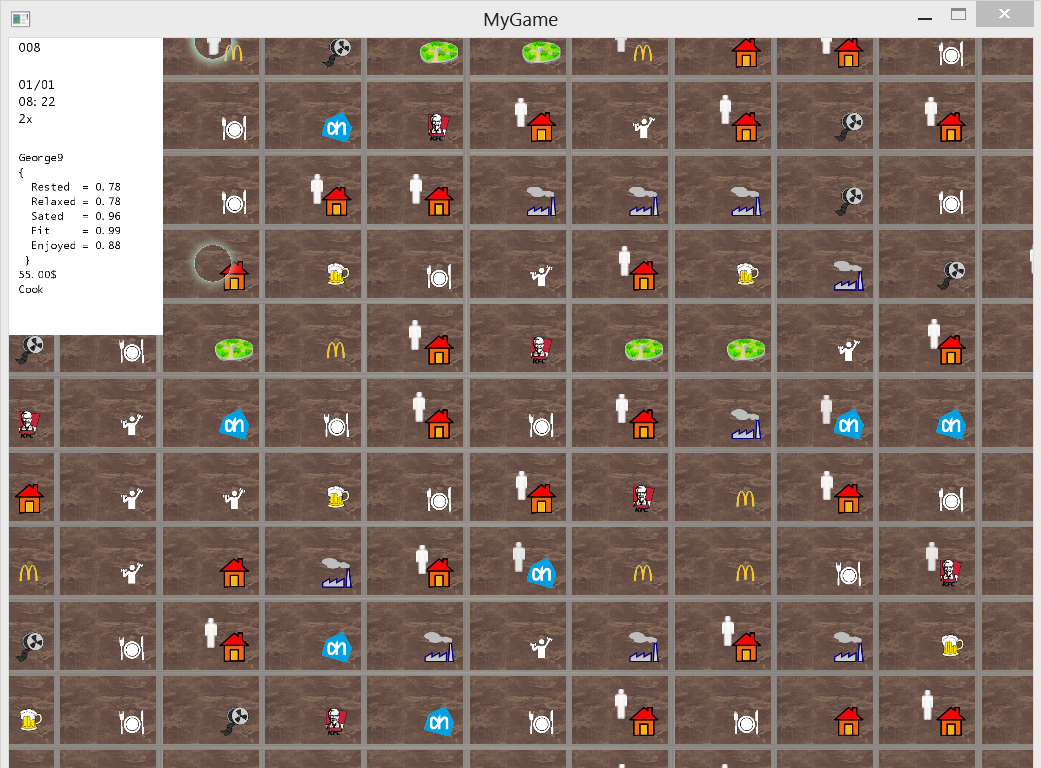
\includegraphics[width=6cm]{Pics/big_city.png}
\caption{The first virtual city}
\label{fig:first_virtual_city}
\end{figure}
}\end{textslide}

\begin{frame}{Results}
\center
\fontsize{18pt}{7.2}\selectfont
Virtual city demo
\end{frame}

\begin{textslide}{Results}{Preferences}{
\begin{figure}
\center
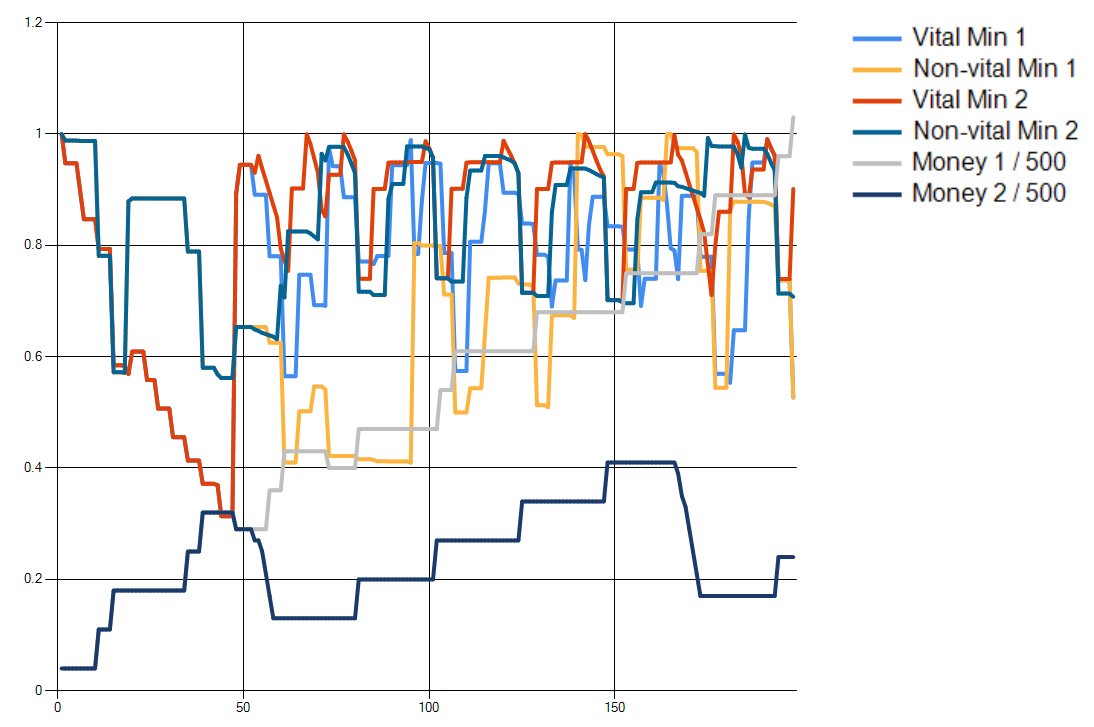
\includegraphics[width=6cm]{Pics/stats_and_money.png}
\caption{The resources of two agents: first with the goal of survival plus earning 500 units of money, second with just the goal of survival}
\label{fig:stats_with_and_without_goal}
\end{figure}
}\end{textslide}

\begin{textslide}{Results}{Preferences}{
\begin{figure}
\center
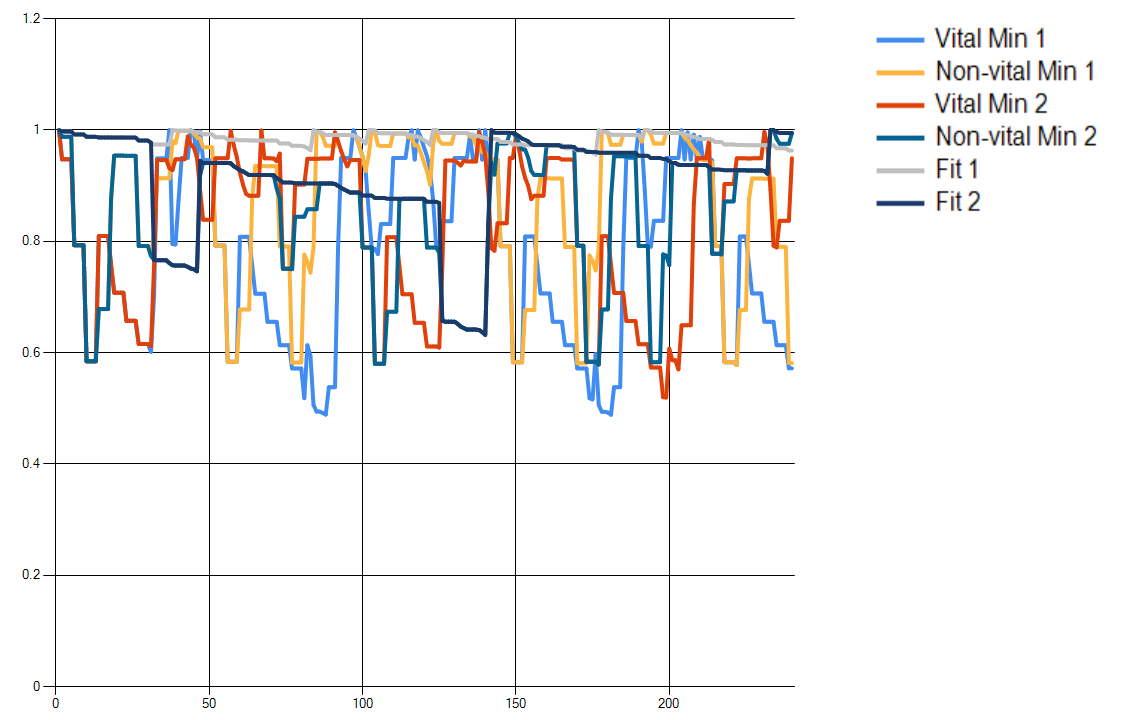
\includegraphics[width=6cm]{Pics/stats_and_fitness.png}
\caption{The resources of two agents: first is a fitness lover, second is a regular NPC}
\label{fig:stats_by_personality}
\end{figure}
}\end{textslide}

\begin{textslide}{Results}{Long-term survival}{
\begin{figure}
\center
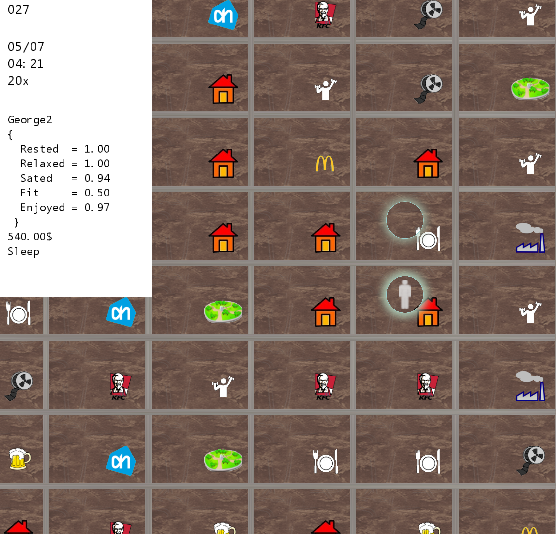
\includegraphics[width=4cm]{Pics/six_months.png}
\caption{Six months survival}
\label{fig:mortality_rate}
\end{figure}
}\end{textslide}

\begin{textslide}{Results}{Scalability}{
\begin{table}
\center
\begin{tabular}{| c | c | c | c |}
\hline
Num agents & City size (sq. km) & FPS & Speedup (min. / sec.) \\
\hline
100 & 6 $\times$ 6 & 30 & 10 \\
150 & 6 $\times$ 6 & 30 & 5 \\
200 & 6 $\times$ 6 & 30 & 5 \\
250 & 7.5 $\times$ 7.5 & 30 & 5 \\
300 & 9 $\times$ 9 & 15 & 2 \\
\hline
\end{tabular}
\caption{Planner performance}
\label{tab:planner_performance}
\end{table}
}\end{textslide}

\section{Conclusions}
\begin{slide}{Conclusions}{Problem}{
\item Use of a layered planning technique in order to create non-playing-characters (NPCs) that \textit{live} in a game world
\item Greatly increases the believability of the game world, and gives additional depth to the game
}\end{slide}

\begin{slide}{Conclusions}{Idea}{
\item Planner inspired from forward-chaining constraint logic programming
\item Aggressive heuristics for steering
\item Aggressive pruning of less promising partial plans
\item Memoization to recycle old but effective plans
\item Using such a system in real-time poses additional challenges of reliability and concurrency
}\end{slide}

\begin{slide}{Conclusions}{Results}{
\item Our technique offers multiple positive features
\item Our layered planner is \textit{fast} and \textbf{effective}
\item It guides hundreds of NPCs to survival in challenging, real-time scenarios for long periods of time
\item NPC survive indefinitely
}\end{slide}

\begin{slide}{Conclusions}{Results}{
\item \textbf{General-purpose} planner
\begin{itemize}
\item Parametrized set of actions
\item Parametrized environment
\end{itemize}
\item The behaviors of our NPCs reach short-, medium-, and long term \textit{goals}
\item NPCs are \textit{customizable}
}\end{slide}

\begin{frame}{That's it}
\center
\fontsize{18pt}{7.2}\selectfont
Thank you!
\end{frame}

\begin{frame}[allowframebreaks]
\frametitle{References}
\bibliographystyle{plain}
\bibliography{bibliography}
\end{frame}

\end{document}
